
\documentclass[letterpaper,UKenglish]{lipics-v2018}
\usepackage{tikz-cd}
\usepackage{hyperref}

%\usepackage{microtype}%if unwanted, comment out or use option "draft"

%\graphicspath{{./graphics/}}%helpful if your graphic files are in another directory

\bibliographystyle{plainurl}% the recommnded bibstyle

\title{Detecting graph isomorphisms using deep learning}

%\titlerunning{Dummy short title}%optional, please use if title is longer than one line

\author{Muzamil Yahia}{University of Hawaii at Manoa}{}{}{}%mandatory, please use full name; only 1 author per \author macro; first two parameters are mandatory, other parameters can be empty.

%\author{Joan R. Public}{Department of Informatics, Dummy College, [Address], Country}{joanrpublic@dummycollege.org}{[orcid]}{[funding]}

\authorrunning{Muzamil Yahia}%mandatory. First: Use abbreviated first/middle names. Second (only in severe cases): Use first author plus 'et al.'

\Copyright{Public}%mandatory, please use full first names. LIPIcs license is "CC-BY";  http://creativecommons.org/licenses/by/3.0/

\subjclass{Models of learning}% mandatory: Please choose ACM 2012 classifications from https://www.acm.org/publications/class-2012 or https://dl.acm.org/ccs/ccs_flat.cfm . E.g., cite as "General and reference $\rightarrow$ General literature" or \ccsdesc[100]{General and reference~General literature}. 

\keywords{Deep learning, graphs, graph automorphism, graph homomorphisms}%mandatory

%\category{Class Project}%optional, e.g. invited paper

%\relatedversion{}%optional, e.g. full version hosted on arXiv, HAL, or other respository/website

\supplement{}%optional, e.g. related research data, source code, ... hosted on a repository like zenodo, figshare, GitHub, ...

%\funding{}%optional, to capture a funding statement, which applies to all authors. Please enter author specific funding statements as fifth argument of the \author macro.

%\acknowledgements{I want to thank \dots}%optional

%Editor-only macros:: begin (do not touch as author)%%%%%%%%%%%%%%%%%%%%%%%%%%%%%%%%%%
\EventEditors{John Q. Open and Joan R. Access}
\EventNoEds{2}
\EventLongTitle{42nd Conference on Very Important Topics (CVIT 2016)}
\EventShortTitle{ICS691C 2018}
\EventAcronym{}
\EventYear{2018}
\EventDate{December 8, 2018}
\EventLocation{Hawaii, US}
\EventLogo{}
\SeriesVolume{42}
\ArticleNo{1}

%\nolinenumbers %uncomment to disable line numbering
%\hideLIPIcs  %uncomment to remove references to LIPIcs series (logo, DOI, ...), e.g. when preparing a pre-final version to be uploaded to arXiv or another public repository
%%%%%%%%%%%%%%%%%%%%%%%%%%%%%%%%%%%%%%%%%%%%%%%%%%%%%%
\nolinenumbers

\begin{document}

\maketitle

\begin{abstract}
This project aims to detect graph isomorphism from a given graph. We first generate a bunch of isomorphic graphs and non isomorphic graphs as our data. We train our neural network using these data, and then test and state the loss and accuracy.
\end{abstract}


\section{Introduction}
A \emph{directed} graph $G \equiv (V,E)$ can be written as a mapping $G \equiv \begin{tikzcd} E \arrow[r,"\rho",swap] \arrow[r,"\delta",shift left = .8ex]& V \end{tikzcd}$ where $\delta(e)$ and $\rho(e)$ indicate the source and destination for each edge $e \in E$. A neighbour of a vertex $v \in V$ is given by the set of vertices $N(v) = \{\, w \in V \mid \exists e \in E. \,  \delta(e) = v \wedge \rho(e) = w   \,\}$ and we say $w$ is adjacent to $v$ if $w \in N(v)$. Undirected graphs add the following restriction $w \in N(v) \implies v \in N(w)$ on $E$.

A graph isomorphism over $G$ is a permutation $p \colon V \to V$ that preserves the adjacency of vertices i.e. $ w \in N(v) \Leftrightarrow p(w) \in N(p(v))$. Checking whether two graphs $g$ and $g'$ are isomorphic amounts to find such permutation. 

\section{Testing for isomorphisms}
Given two graphs $G \equiv \begin{tikzcd} E \arrow[r,"\delta",swap] \arrow[r,"\delta",shift left = .8ex]& V \end{tikzcd}$ and $G' \equiv \begin{tikzcd} E' \arrow[r,"\delta'",swap] \arrow[r,"\rho'",shift left = .8ex]& V' \end{tikzcd}$ . If $V \neq V'$, or $E \neq E'$ i.e. different sizes of vertices or edges, then two graphs are trivially non-isomorphic. The case $|E| = |E'| \wedge |V| = |V'|$ is much harder and in the worst case we may try all permutations $p \colon V \to V'$ and test whether a bijection $e_p\colon E \to E'$ induced by $p$, will provide an isomorphism.

The Graph Isomorphism is an NP-hard problem, and it is not known if it is NP-complete. It is also not known if belongs to co-NP. The fast known result for solving graph isomorphism which stood for 3 decades is $e^{O(\sqrt{n \log n})}$ by Babai et al. \cite{BabaiL83}. However for some special cases of graphs i.e. class of graphs with a forbidden minor and classes of graphs of a topological minor are shown to be solved in polynomial time by Grohe in 2013 \cite{Grohe13}, however these methods are not very useful in practice.

Most common practical algorithms that detect isomorphisms rely on ``canonical relabelling" which takes an advantage of an invariant property of graph isomorphisms; If two graphs are isomorphic then they have the same canonical relabelling. The most successful approach uses a method of fixing a vertex $v$ and then refining the set partitions of $V$ through a strategy called ``individualization and refinement" \cite{parris1969coding}. The method was implemented by McKay in 1979 in C, in a software package named ``Nauty". The software has seen many improvements through the decades and recent improvement was done by 
McKay and Piperno in 2014 in a new software called ``Tracy" \cite{mckay2014practical}.

\section{Deep learning and graph isomorphism}
Since the graph isomorphism problem is NP-hard, we might want to look for heuristic methods to determine whether two graphs are isomorphic for majory of graphs. As neural network has shown recently the ability to learn complicated features hidden in a given set of data, and with careful construction of these networks, they can be generalized to unseen data input. Therefore, a classifier neural network would be a suitable choice for detecting graph isomoprhism. We will specify our methods in the subsections below.

\subsection{Problem statement}
Given a graph $G = (V,E)$, find a neural network model that can receive as input a graph $G' = (V',E')$, check if $G$ is isomorphic to $G'$ with high probability.  

\subsection{Method}
We encode the graph $G$ using adjacency matrix, and produce $m$ isomorphic graphs $\{ G' \mid G' \cong G \}$. To do that, we take to our advantage the simple forward approach and generate a random permutation of vertices $p \colon V\to V$, and then rewrite the adjacency matrix to reflect that as shown the diagram below:

\begin{tikzcd}
v \arrow[r,"p",dashed] \arrow[d,"e"] & p(v) \arrow[d,"e_p"]\\
w \arrow[r,"p",dashed] & p(w)   
\end{tikzcd}

To generate non isomorphic data, we followed a simple approach first by reducing the set $E$ by randomly removing one edge, and later removing random number of edges. 

I note that this approach of non-isomorphism is trivial, and does not tackle the heart of the problem. Future work would be to generate all isomorphisms graphs using Nauty/Tracy packages and then use these data for training and testing. For now I will focus only on the trivial case of changing the size of edges $E$.

\subsection{Results}
Sequential neural network struggled to learn effectively for some large set of edges and learnt effectively for smaller sets. Figure \ref{figureseq} shows loss and accuracy for a sequential neural network of 8 layers. The accuracy is higher for 10--20 edges but then get lower and lower for rest of 20--120 edges.

Convolutional neural network with two covoluted layers did the opposite. For small set of edges 10--50 the model showed little accuracy. However, for larger set of edges 60--120, the convoluted model showed better accurcay in training and also in validation. 

\section{Conclusion and future work}
Graph isomorphism is an NP-hard problem which might be tackled with tools of deep-learning. Sequential models were effective for only small set of edges, while convolutional network worked better for graphs that are more than half-full. In future work, we would implement combinations of graph of same number of edges, graphs with different sizes, and also graph homomorphisms.

\begin{figure}\label{figseq}
\centering
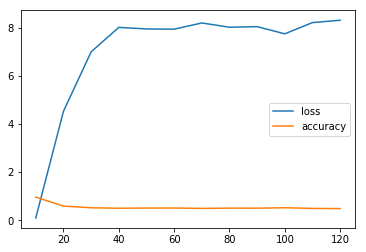
\includegraphics[scale = .5]{pic/8-layers-sequential}
\caption{Loss and accuracy for a sequential neural network of 8 layers and 6 epochs. The underlying graphs consists of 16 nodes and edges from the set $\{10,20, \dots, 120 \}$.}
\end{figure}

\begin{figure}
\centering
  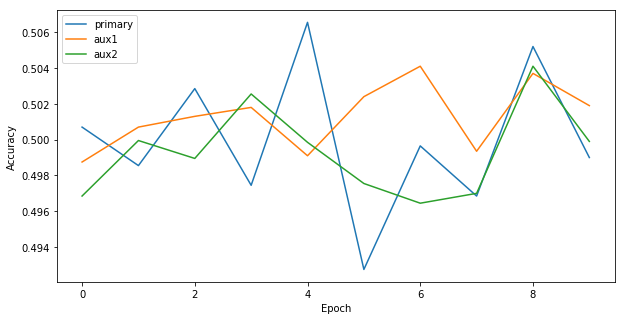
\includegraphics[scale = .5]{pic/10-edges-conv.png}
\caption{Loss and accuracy for a convolutional neural network of 2 convolutional layers and 10 epochs. The underlying graphs consists of 16 nodes and 10 edges.}
\end{figure}

\begin{figure}
\centering
  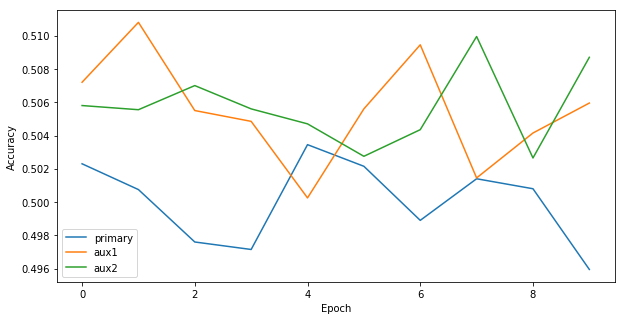
\includegraphics[scale = .5]{pic/20-edges-conv.png}
\caption{Loss and accuracy for a convolutional neural network of 2 convolutional layers and 10 epochs. The underlying graphs consists of 16 nodes and 20 edges.}
\end{figure}

\begin{figure}
\centering
  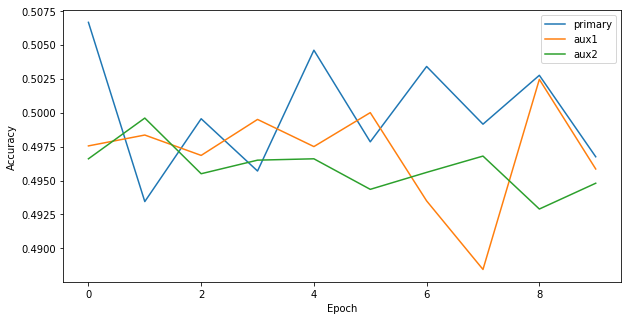
\includegraphics[scale = .5]{pic/30-edges-conv.png}
\caption{Loss and accuracy for a convolutional neural network of 2 convolutional layers and 10 epochs. The underlying graphs consists of 16 nodes and 30 edges.}
\end{figure}

\begin{figure}
\centering
  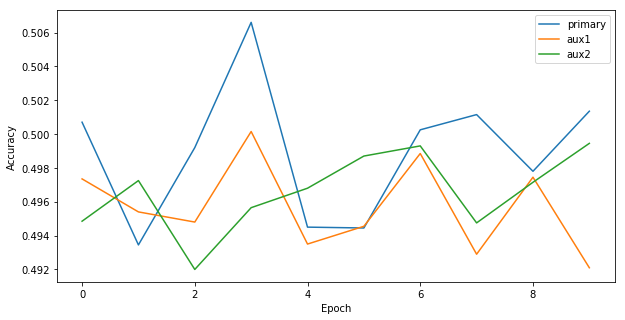
\includegraphics[scale = .5]{pic/40-edges-conv.png}
\caption{Loss and accuracy for a convolutional neural network of 2 convolutional layers and 10 epochs. The underlying graphs consists of 16 nodes and 40 edges.}
\end{figure}

\begin{figure}
\centering
  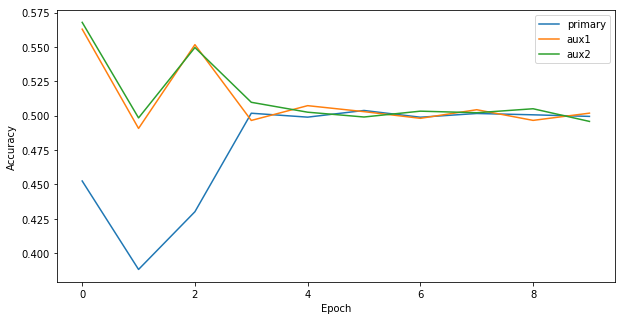
\includegraphics[scale = .5]{pic/50-edges-conv.png}
\caption{Loss and accuracy for a convolutional neural network of 2 convolutional layers and 10 epochs. The underlying graphs consists of 16 nodes and 50 edges.}
\end{figure}

\begin{figure}
\centering
  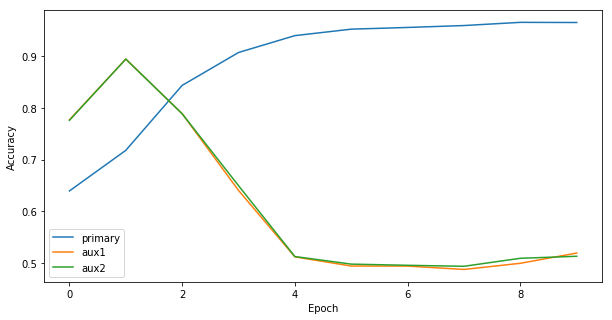
\includegraphics[scale = .5]{pic/60-edges-conv.png}
\caption{Loss and accuracy for a convolutional neural network of 2 convolutional layers and 10 epochs. The underlying graphs consists of 16 nodes and 60 edges.}
\end{figure}

\begin{figure}
\centering
  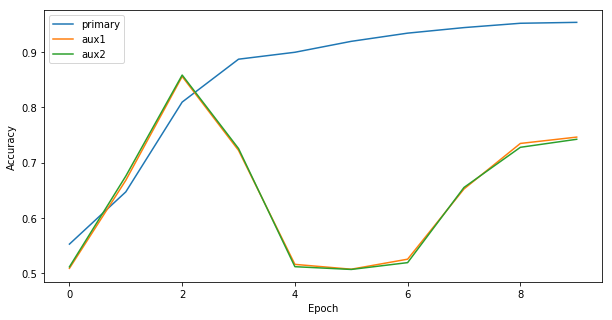
\includegraphics[scale = .5]{pic/70-edges-conv.png}
\caption{Loss and accuracy for a convolutional neural network of 2 convolutional layers and 10 epochs. The underlying graphs consists of 16 nodes and 70 edges.}
\end{figure}

\begin{figure}
\centering
  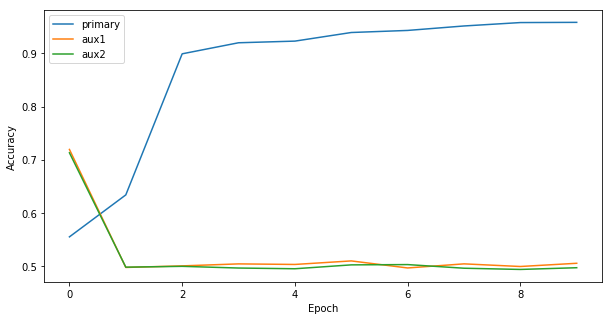
\includegraphics[scale = .5]{pic/80-edges-conv.png}
\caption{Loss and accuracy for a convolutional neural network of 2 convolutional layers and 10 epochs. The underlying graphs consists of 16 nodes and 80 edges.}
\end{figure}

\begin{figure}
\centering
  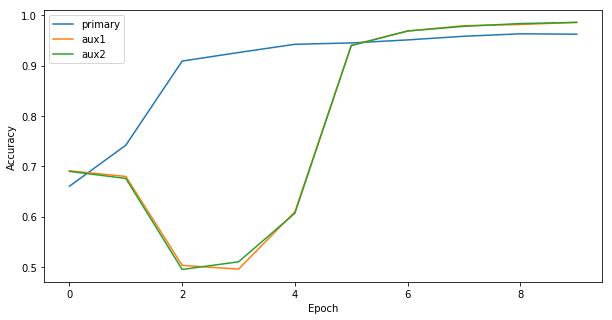
\includegraphics[scale = .5]{pic/90-edges-conv.png}
\caption{Loss and accuracy for a convolutional neural network of 2 convolutional layers and 10 epochs. The underlying graphs consists of 16 nodes and 90 edges.}
\end{figure}

\begin{figure}
\centering
  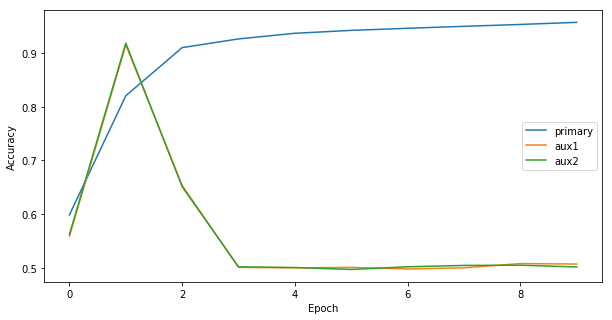
\includegraphics[scale = .5]{pic/100-edges-conv.png}
\caption{Loss and accuracy for a convolutional neural network of 2 convolutional layers and 10 epochs. The underlying graphs consists of 16 nodes and 100 edges.}
\end{figure}

\begin{figure}
\centering
  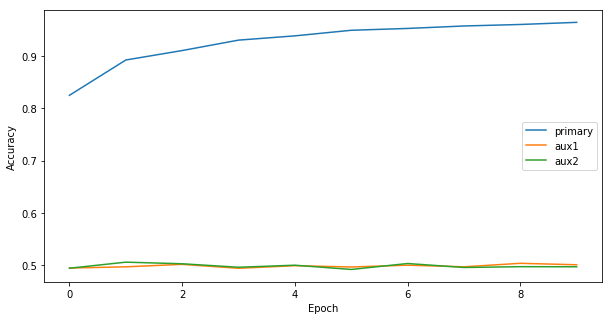
\includegraphics[scale = .5]{pic/110-edges-conv.png}
\caption{Loss and accuracy for a convolutional neural network of 2 convolutional layers and 10 epochs. The underlying graphs consists of 16 nodes and 110 edges.}
\end{figure}

\begin{figure}
\centering
  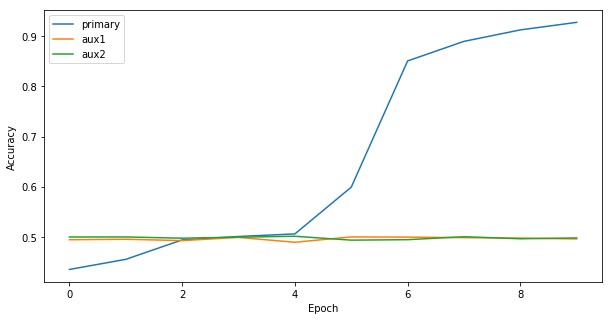
\includegraphics[scale = .5]{pic/120-edges-conv.png}
\caption{Loss and accuracy for a convolutional neural network of 2 convolutional layers and 10 epochs. The underlying graphs consists of 16 nodes and 120 edges.}
\end{figure}

\bibliography{lipics-v2018-sample-article}

\end{document}